\documentclass[11pt,a4paper]{article}

\usepackage[utf8]{inputenc}
\usepackage[T1]{fontenc}
\usepackage{lmodern}
\usepackage[english]{babel}
\usepackage[a4paper,margin=2.5cm]{geometry}
\usepackage{amsmath,amssymb}
\usepackage{graphicx}
\usepackage{booktabs}
\usepackage{hyperref}
\usepackage{float}
\usepackage{caption}
\usepackage{enumitem}
\graphicspath{{./figures/}}

\title{Molecular Geometry from Repelling Nodes on a Sphere: A Minimal Energy Approach}
\author{Vladimir Yakovlev}
\date{March 2026}

\begin{document}
\maketitle

\begin{abstract}
We present a minimal geometric model in which molecular-like shapes emerge from repelling nodes constrained to a sphere. Instead of introducing separate rules for orbitals, hybridization, or allowed molecular forms, the model uses only two node types, a repulsion parameter, and spherical energy minimization. The resulting configurations reproduce familiar small-$N$ geometries, exhibit a soft octahedral regime at $N=6$, develop geometric degeneracy and pentagonal motifs at $N=7$, and reach a stable icosahedral-like packing at $N=12$. The value of the approach lies not in adding new rules, but in reducing the number of assumptions needed to recover known forms.
\end{abstract}

\section{Introduction}
Molecular geometry is commonly described through a combination of empirical rules and semi-empirical language: electron pairs, lone pairs, hybridization patterns, allowed forms, and their corresponding exceptions. This vocabulary is useful in practice, but it also raises a methodological question: how much of the familiar geometric structure can be recovered from a smaller set of assumptions?

In this work, we study a minimal geometric model in which interacting nodes are constrained to lie on a sphere. The model uses only two node types, denoted $B$ and $L$, a repulsion parameter $\alpha$, and numerical minimization of an energy-like functional. No separate rules for tetrahedral, trigonal bipyramidal, octahedral, or other standard molecular geometries are introduced. When such forms appear, they arise as minima of the same optimization problem.

The goal of the model is limited and specific. It is not intended as a complete theory of chemical bonding. Rather, it serves as a geometric baseline: a test of how far one can go while keeping the descriptive language as simple as possible. In this sense, the interest of the model lies not in introducing a richer framework, but in determining whether familiar structures can emerge from fewer independent assumptions.

The results define a coherent sequence. At small $N$, the model reproduces standard VSEPR-like geometries. At $N=6$, it enters a soft octahedral regime rather than a single rigid ideal form. At $N=7$, geometric degeneracy appears together with pentagonal motifs. Finally, a probe test at $N=12$ yields a robust icosahedral-like packing. Taken together, these cases suggest that a substantial part of the usual geometric rulebook may be replaced by a single organizing principle: spherical energy minimization of interacting nodes.

\section{Minimal model}

\subsection{Degrees of freedom}
The configuration consists of $N$ nodes constrained to the unit sphere, with
\[
N = N_B + N_L,
\]
where $N_B$ is the number of bonding centres ($B$) and $N_L$ is the number of lone centres ($L$).

Each configuration is defined by:
\begin{itemize}[leftmargin=1.5em]
    \item the total number of nodes $N$,
    \item the composition $(N_B, N_L)$,
    \item the node positions on the sphere,
    \item the interaction parameter $\alpha$.
\end{itemize}

\subsection{Interaction and control parameter}
The model uses a single effective parameter $\alpha$ controlling the relative strength of repulsion in the optimization functional. In version~1, $\alpha$ is treated as an external control parameter rather than a quantity derived from a deeper physical model.

\subsection{Optimization}
For fixed $(N_B, N_L, \alpha)$, the configuration is obtained numerically by repeated restarts followed by local minimization. The best minimum found across all restarts is retained as the representative configuration.

The basic diagnostics recorded for each run are:
\begin{itemize}[leftmargin=1.5em]
    \item best energy,
    \item full angle statistics,
    \item type-resolved angle statistics,
    \item Cartesian coordinates of the optimized points.
\end{itemize}

\subsection{Scope of version 1}
Version~1 is deliberately restricted to geometry. It does not attempt to encode orbital structure, explicit charge distributions, or a full microscopic theory of chemical bonding. Its purpose is to test how much of the standard geometric repertoire can arise from a sparse and uniform set of assumptions.

\section{Reference validation: \texorpdfstring{$N=5$}{N=5}}
The first reference case is the configuration
\[
N=5, \qquad N_B=2, \qquad N_L=3.
\]
In standard VSEPR notation, this corresponds to \(AX_2E_3\).

The optimized geometry reproduces the familiar trigonal bipyramidal arrangement, with the characteristic angle pattern
\begin{itemize}[leftmargin=1.5em]
    \item $BB \approx 180^\circ$,
    \item $BL \approx 90^\circ$,
    \item $LL \approx 120^\circ$.
\end{itemize}

This case is important because no trigonal-bipyramidal rule is imposed separately. The geometry appears directly as the minimum of the same spherical optimization problem used throughout the model. It therefore serves as the reference validation for version~1.

\begin{figure}[H]
    \centering
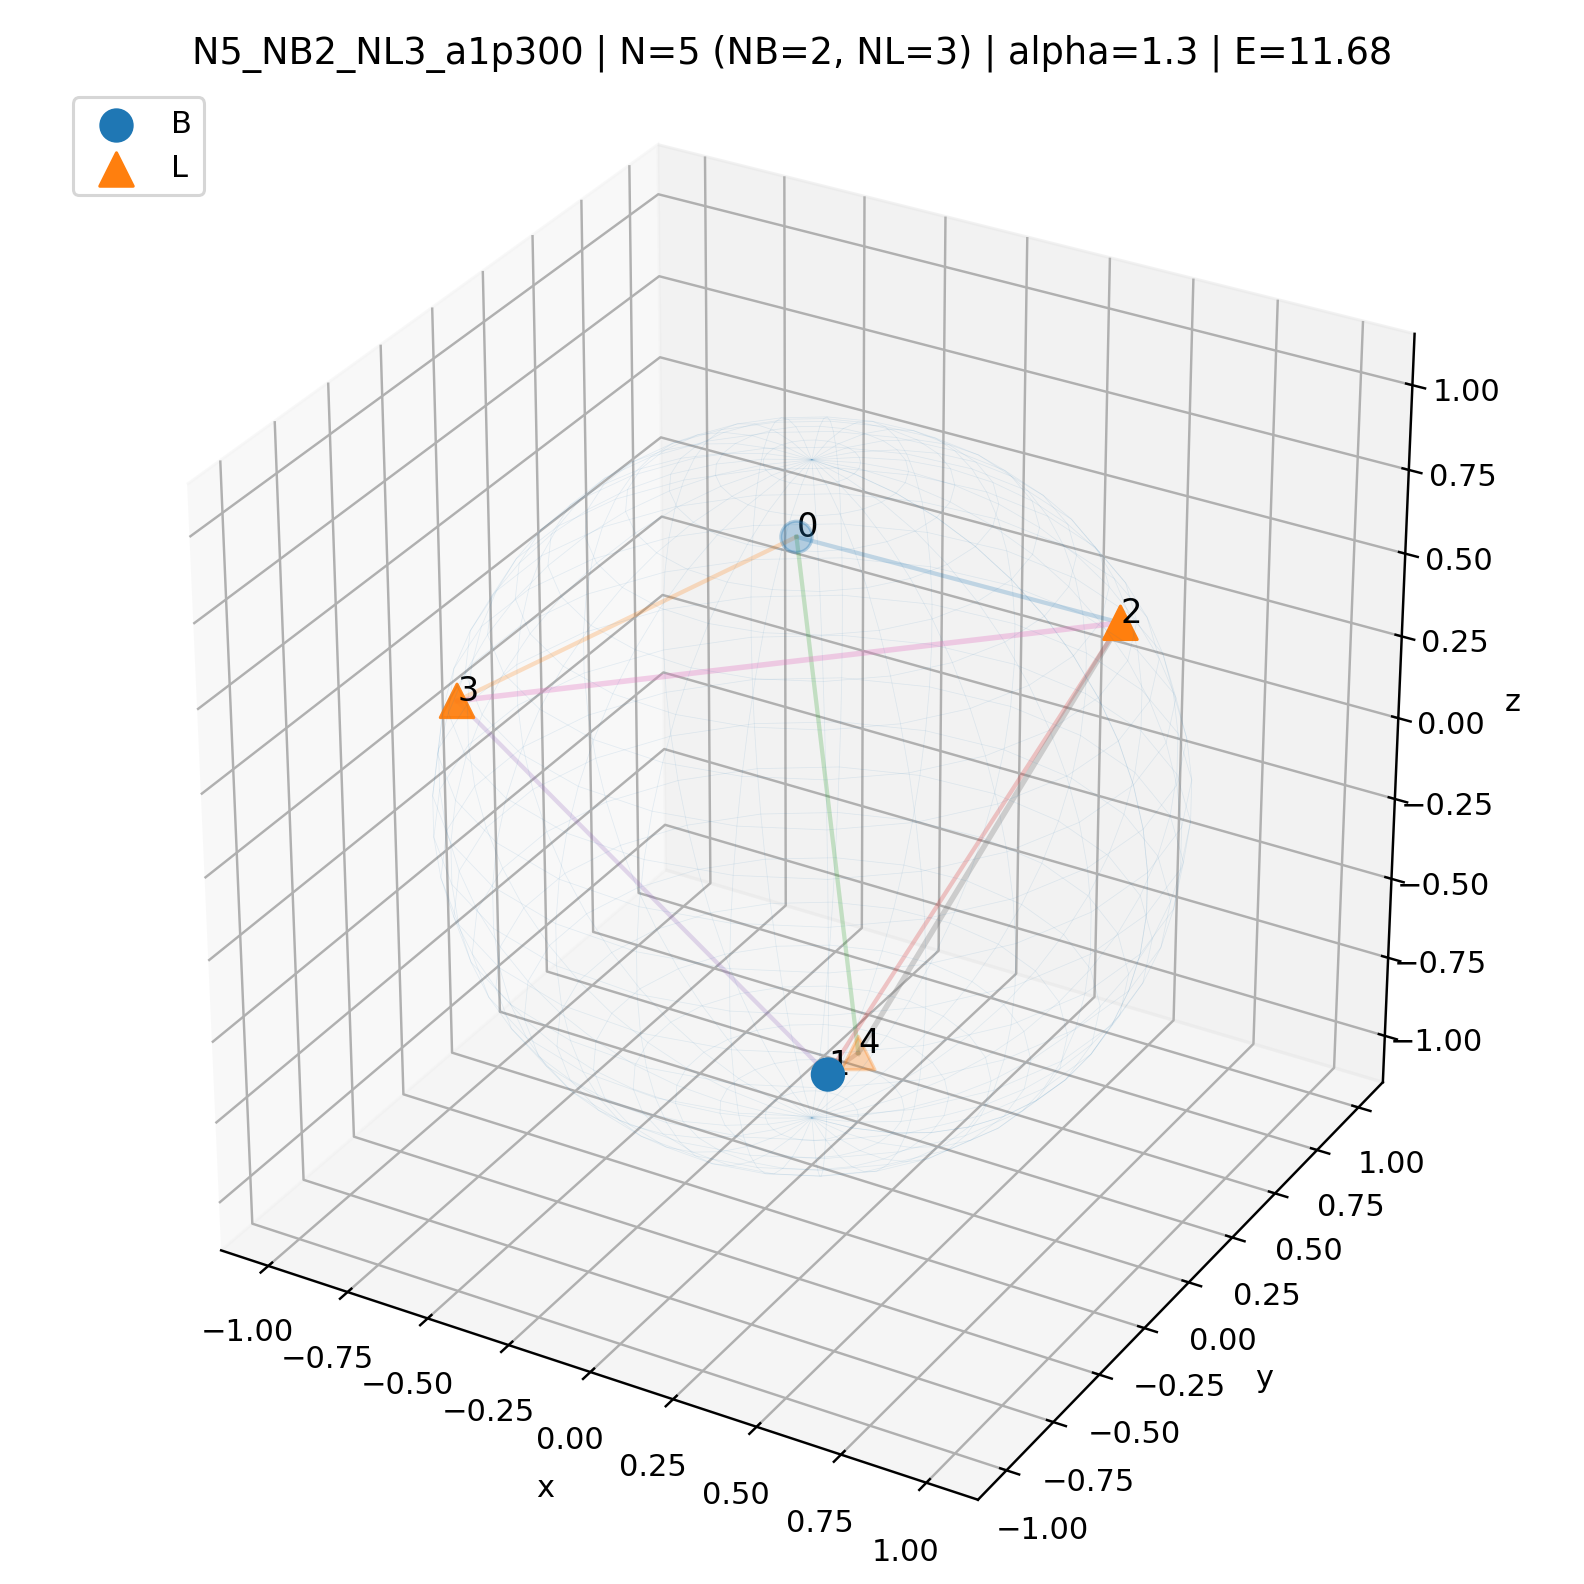
\includegraphics[width=0.78\textwidth]{figures/n5_reference_final.png}
\caption{Reference $N=5$ configuration for the $AX_2E_3$-type case in the minimal sphere model. The optimized arrangement reproduces the expected trigonal-bipyramidal motif from energy minimization alone.}
    \label{fig:n5-reference}
\end{figure}

\section{Soft octahedral regime: \texorpdfstring{$N=6$}{N=6}}
For
\[
N=6, \qquad N_B=2, \qquad N_L=4,
\]
a full scan over $\alpha$ shows a stable regime close to the octahedral geometry. The energy remains stable across runs, the angle statistics vary smoothly with $\alpha$, and no sharp phase transition is observed.

The important point is that this case is better described as a \emph{soft octahedral regime} than as a single rigid ideal octahedron. The geometry remains organized and recognizable, but is not locked into one perfectly discrete form.

\begin{figure}[H]
    \centering
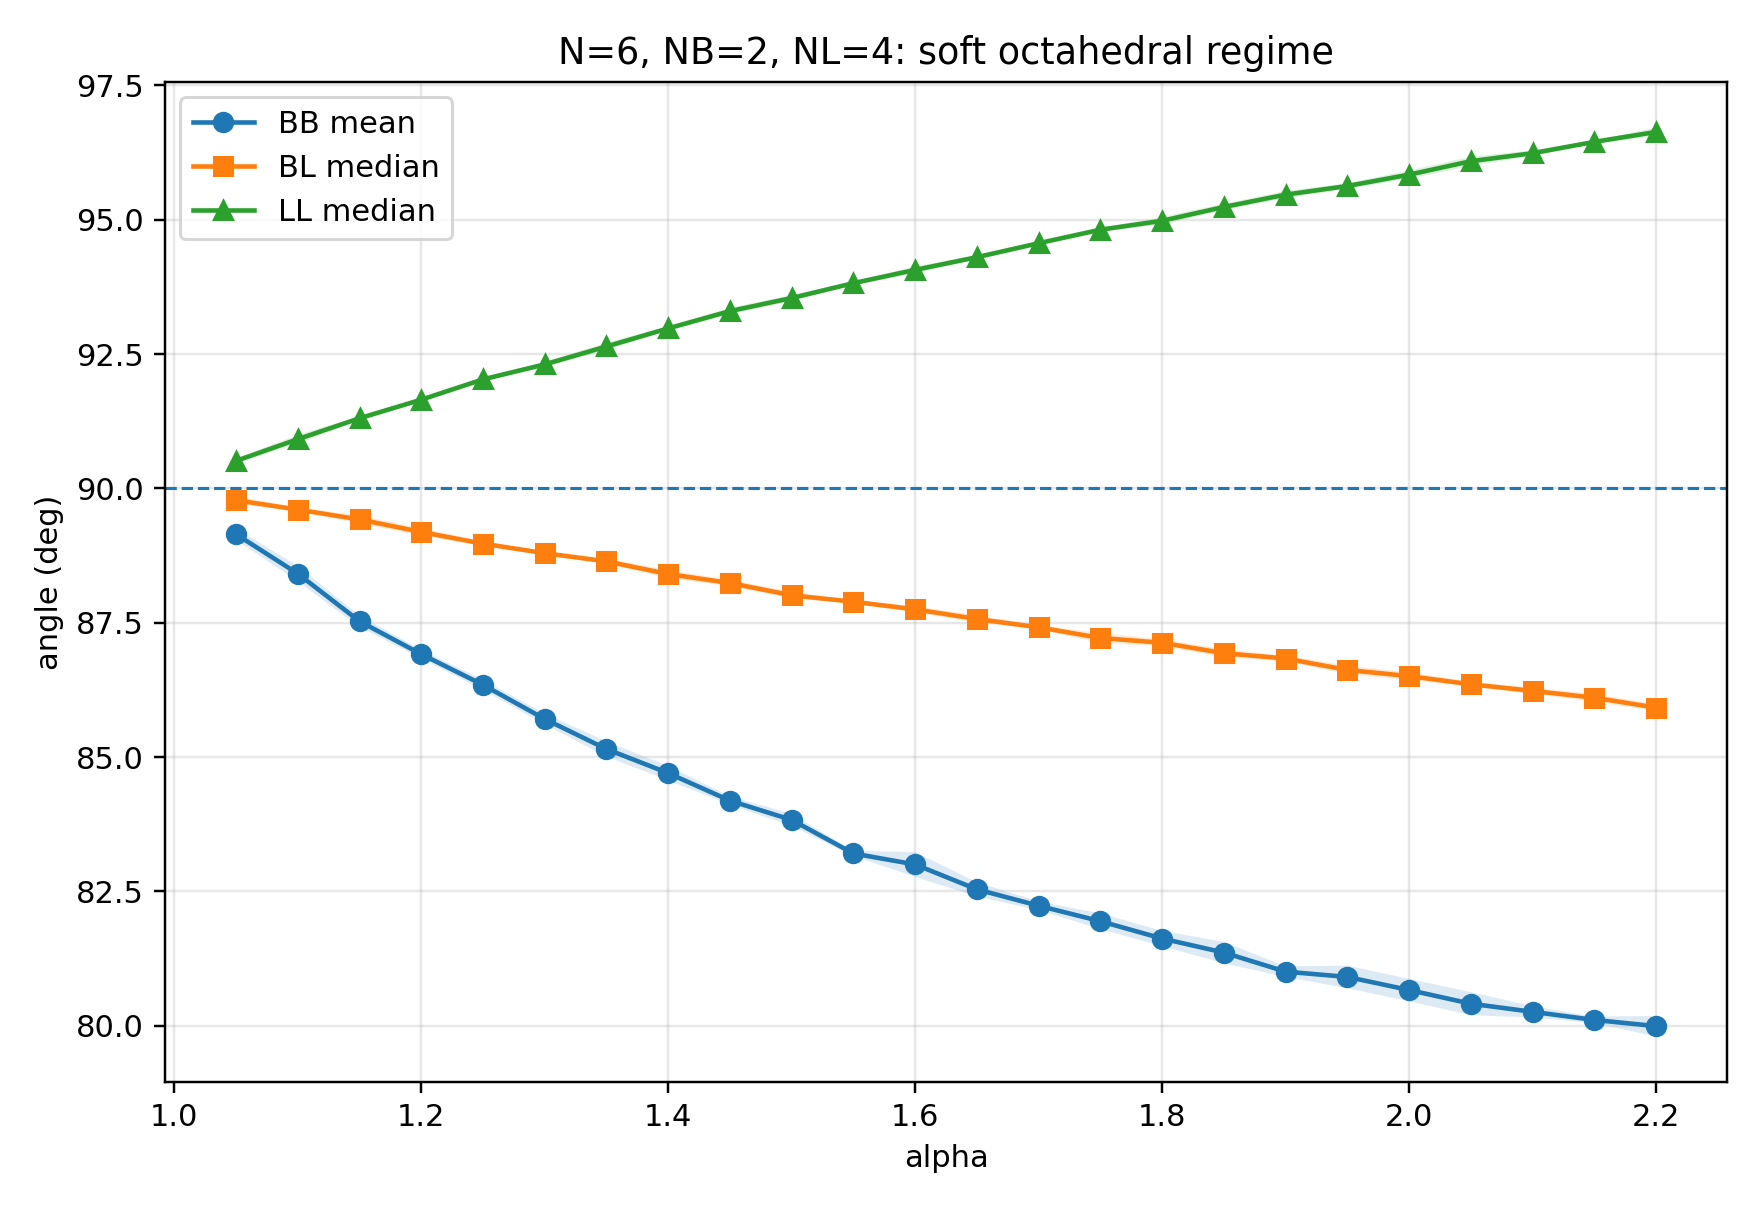
\includegraphics[width=0.82\textwidth]{figures/n6_phase_map.png}
\caption{Angle trends across the $N=6$, $NB=2$, $NL=4$ map. The characteristic angles remain close to the octahedral regime over the scanned $\alpha$ range, indicating a soft but persistent octahedral organization.}
    \label{fig:n6-phase}
\end{figure}

\section{Onset of geometric degeneracy: \texorpdfstring{$N=7$}{N=7}}
The central result of version~1 appears at $N=7$. A dataset of 135 runs was collected for three compositions,
\[
(N_B,N_L) \in \{(1,6),(3,4),(5,2)\},
\]
across nine values of $\alpha$ and five seeds per point.

The main observation is that $N=7$ marks the onset of \emph{soft geometric degeneracy}. The minima remain low-energy and reproducible, but the geometry is no longer captured by a single rigid symmetry class.

\subsection{Case \texorpdfstring{$AX_1E_6$}{AX1E6}}
For $N_B=1$ and $N_L=6$, the system shows a regime change as $\alpha$ increases. This is visible in the type-resolved angle statistics and in the corresponding visualizations.

\subsection{Case \texorpdfstring{$AX_3E_4$}{AX3E4}}
For $N_B=3$ and $N_L=4$, the geometry changes smoothly with $\alpha$. This case illustrates continuous geometric deformation rather than abrupt restructuring.

\subsection{Case \texorpdfstring{$AX_5E_2$}{AX5E2}}
For $N_B=5$ and $N_L=2$, the model yields the most expressive configuration in the $N=7$ family. The characteristic angles are approximately
\begin{itemize}[leftmargin=1.5em]
    \item $BB \approx 108^\circ$,
    \item $BL \approx 90^\circ$,
    \item $LL \approx 180^\circ$.
\end{itemize}
This corresponds to a pentagonal belt of $B$-nodes together with two nearly antipodal $L$-nodes. In visual form, this case provides the clearest demonstration that the model develops a genuine pentagonal motif at $N=7$.

\begin{figure}[H]
    \centering
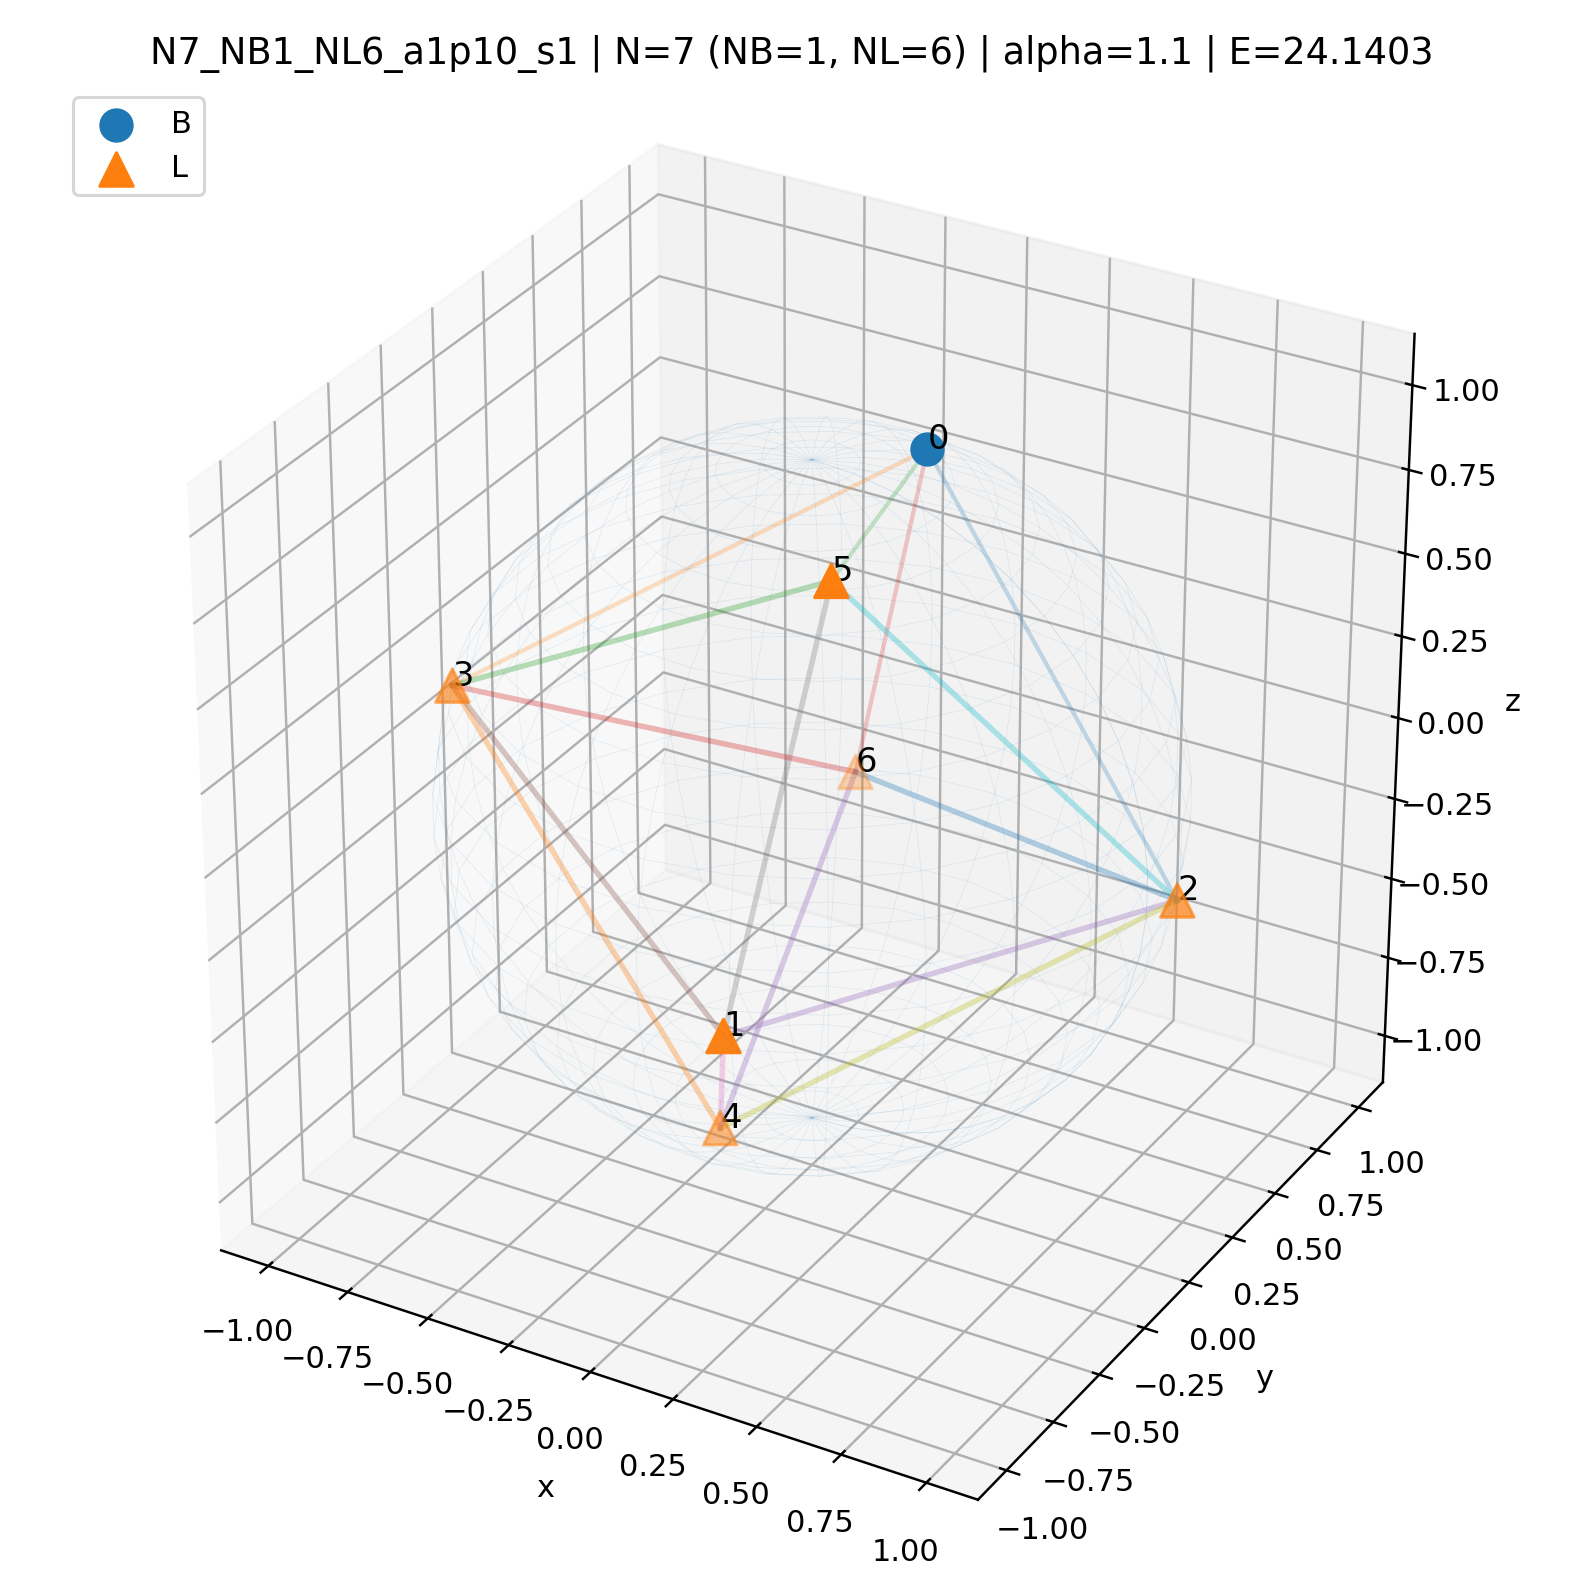
\includegraphics[width=0.78\textwidth]{figures/n7_ax1e6_shift_final.png}
\caption{Representative $N=7$, $AX_1E_6$-type configuration. This case illustrates the onset of geometric softening: the arrangement remains structured, but no longer locks into a single rigid canonical form.}
    \label{fig:n7-ax1e6}
\end{figure}

\begin{figure}[H]
    \centering
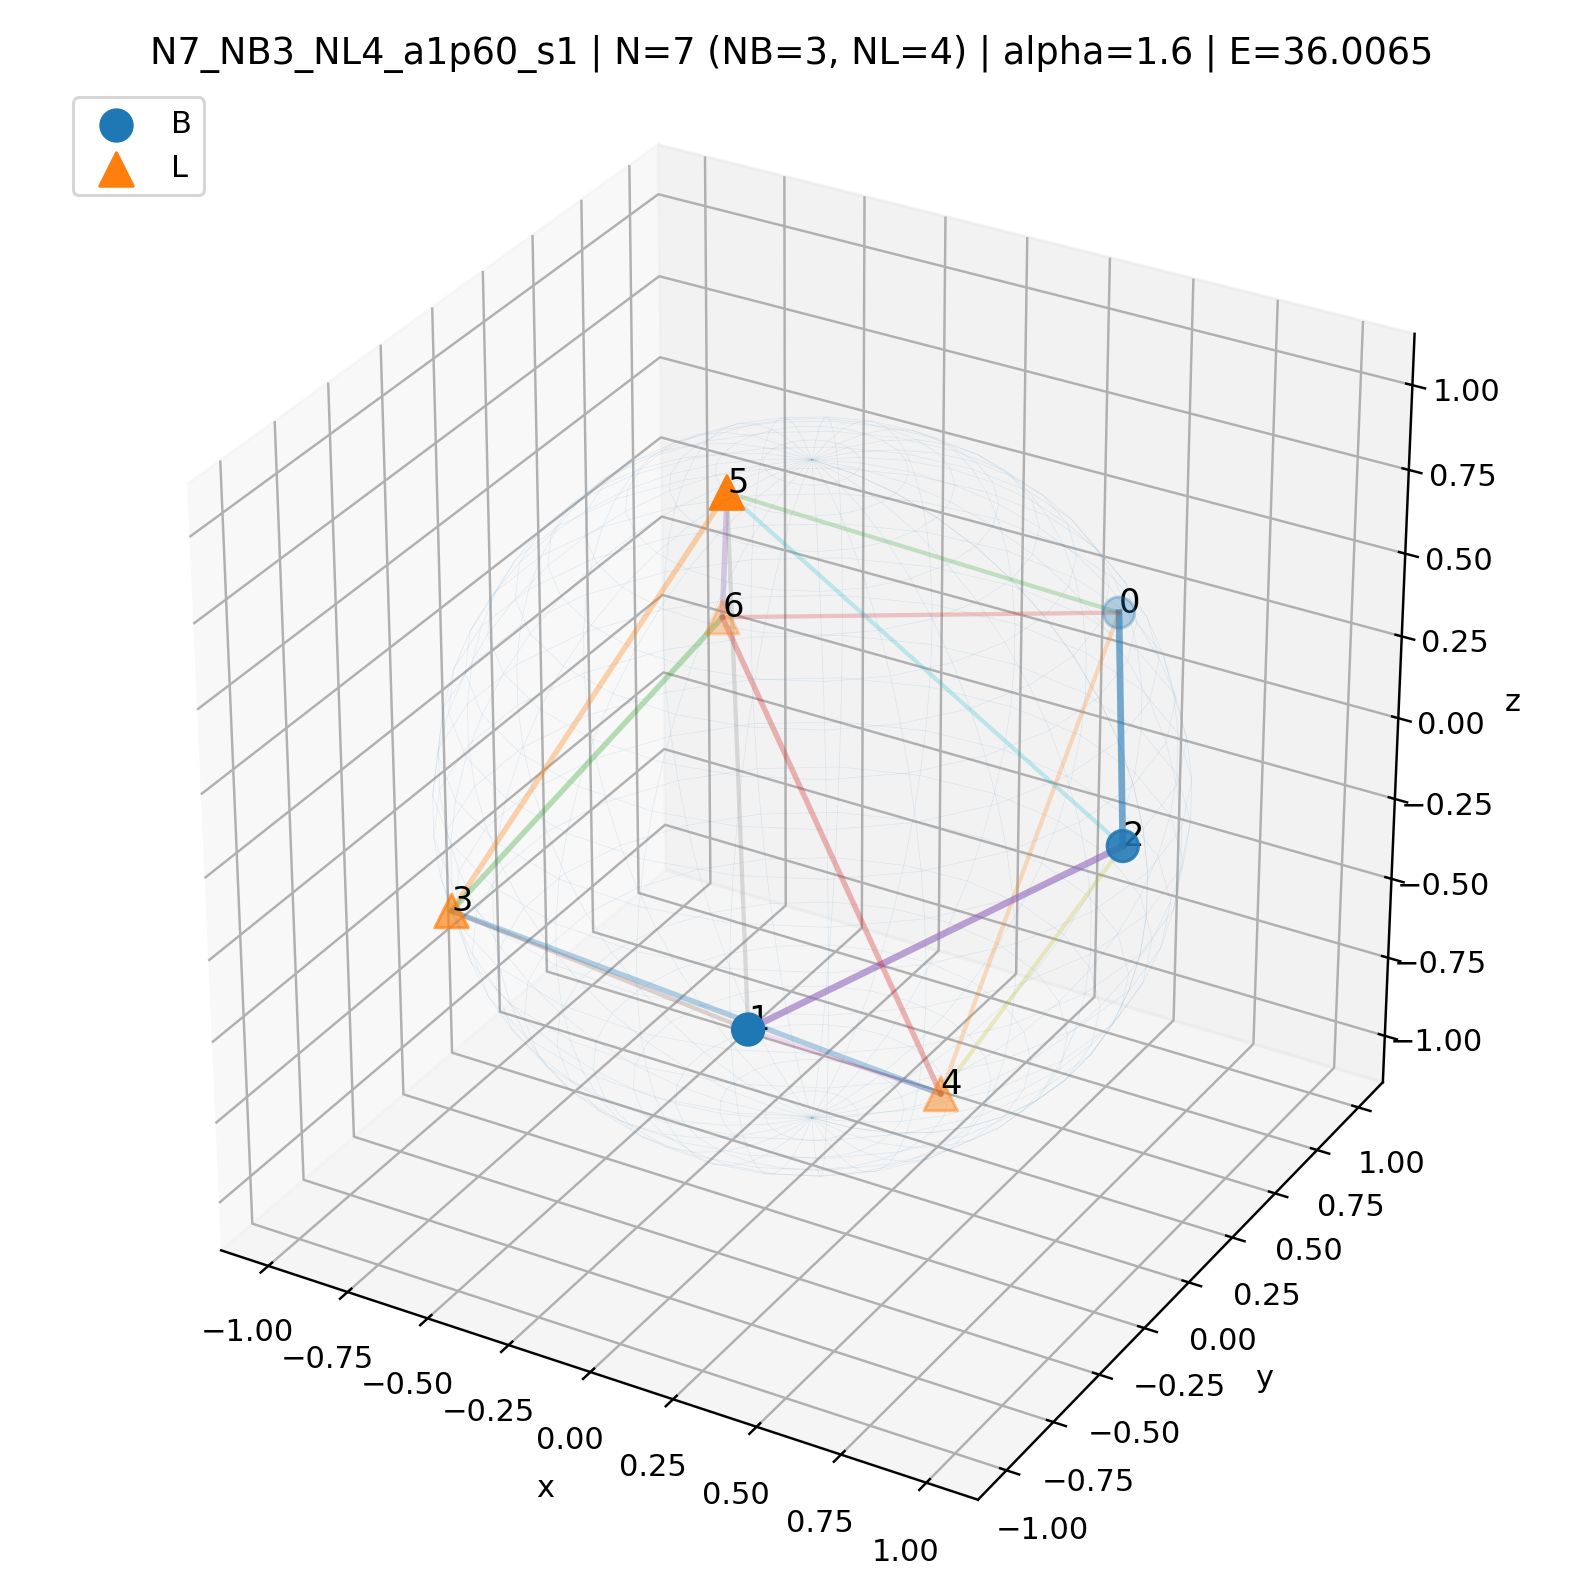
\includegraphics[width=0.78\textwidth]{figures/n7_ax3e4_deformation_final.png}
\caption{Representative $N=7$, $AX_3E_4$-type configuration. The optimized structure shows visible deformation relative to lower-$N$ rigid motifs, consistent with the emergence of soft geometric degeneracy.}
    \label{fig:n7-ax3e4}
\end{figure}

\begin{figure}[H]
    \centering
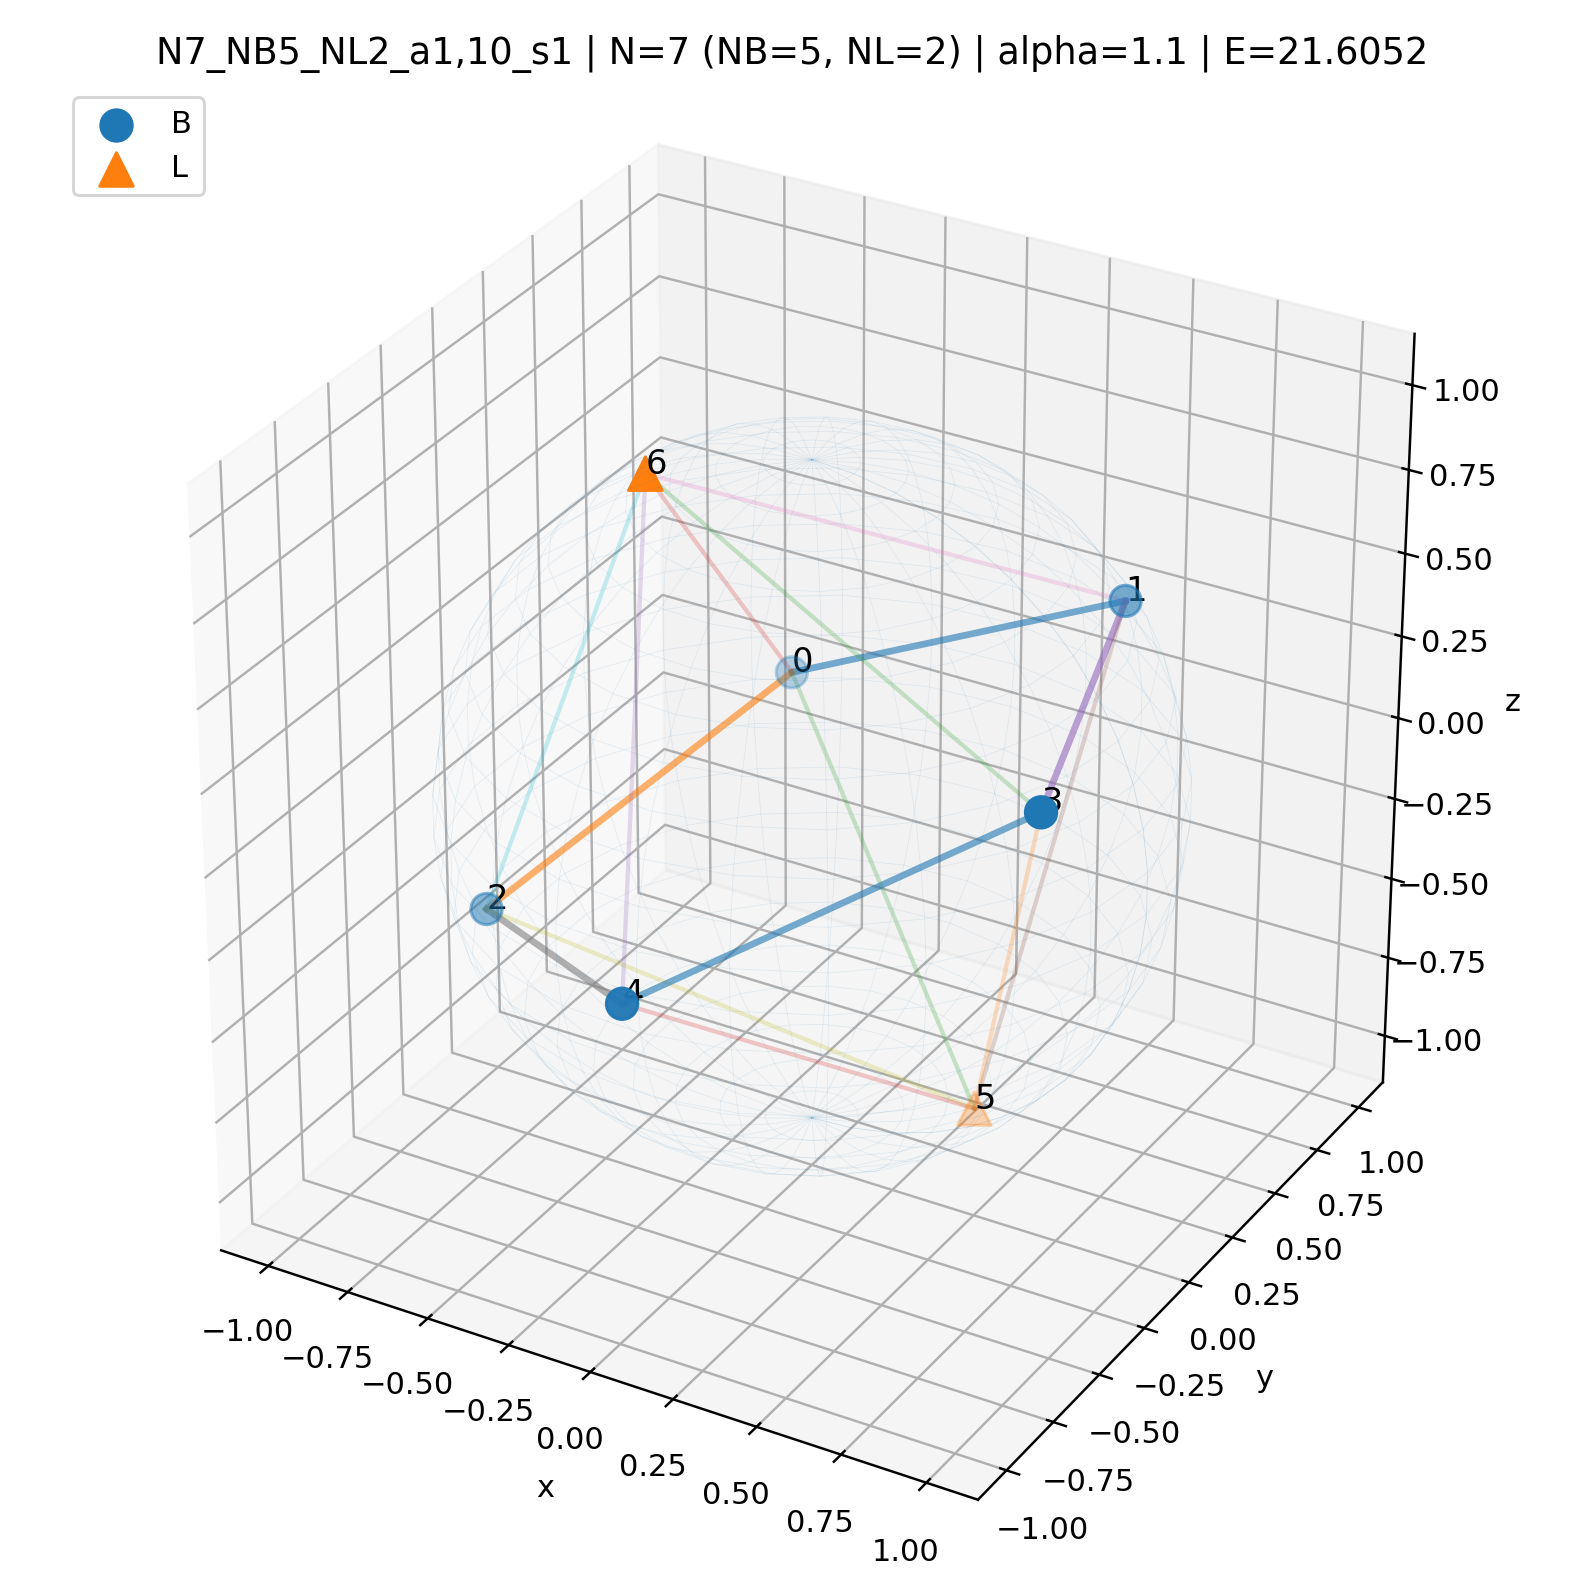
\includegraphics[width=0.78\textwidth]{figures/n7_ax5e2_pentagonal_final.png}
\caption{Representative $N=7$, $AX_5E_2$-type configuration with a pronounced pentagonal motif. This case highlights the appearance of a pentagonal belt structure within the same minimal optimization framework.}
    \label{fig:n7-ax5e2}
\end{figure}

\section{Probe toward icosahedral packing: \texorpdfstring{$N=12$}{N=12}}
As a closing probe, the pure-$B$ case
\[
N=12, \qquad N_B=12, \qquad N_L=0
\]
was tested for several values of $\alpha$ and multiple seeds.

Across all probe runs, the optimized configurations converge to essentially the same angular structure. The characteristic angle distribution is centered around values close to
\begin{itemize}[leftmargin=1.5em]
    \item $63.5^\circ$,
    \item $116^\circ$,
    \item $180^\circ$,
\end{itemize}
with only minor variations between seeds.

This is consistent with a robust icosahedral-like packing on the sphere. In the logic of the present paper, the $N=12$ result is not introduced as a separate main chapter, but as a final probe showing that the same minimal model extends from small VSEPR-like forms to deeper spherical packing structures.

\begin{figure}[H]
    \centering
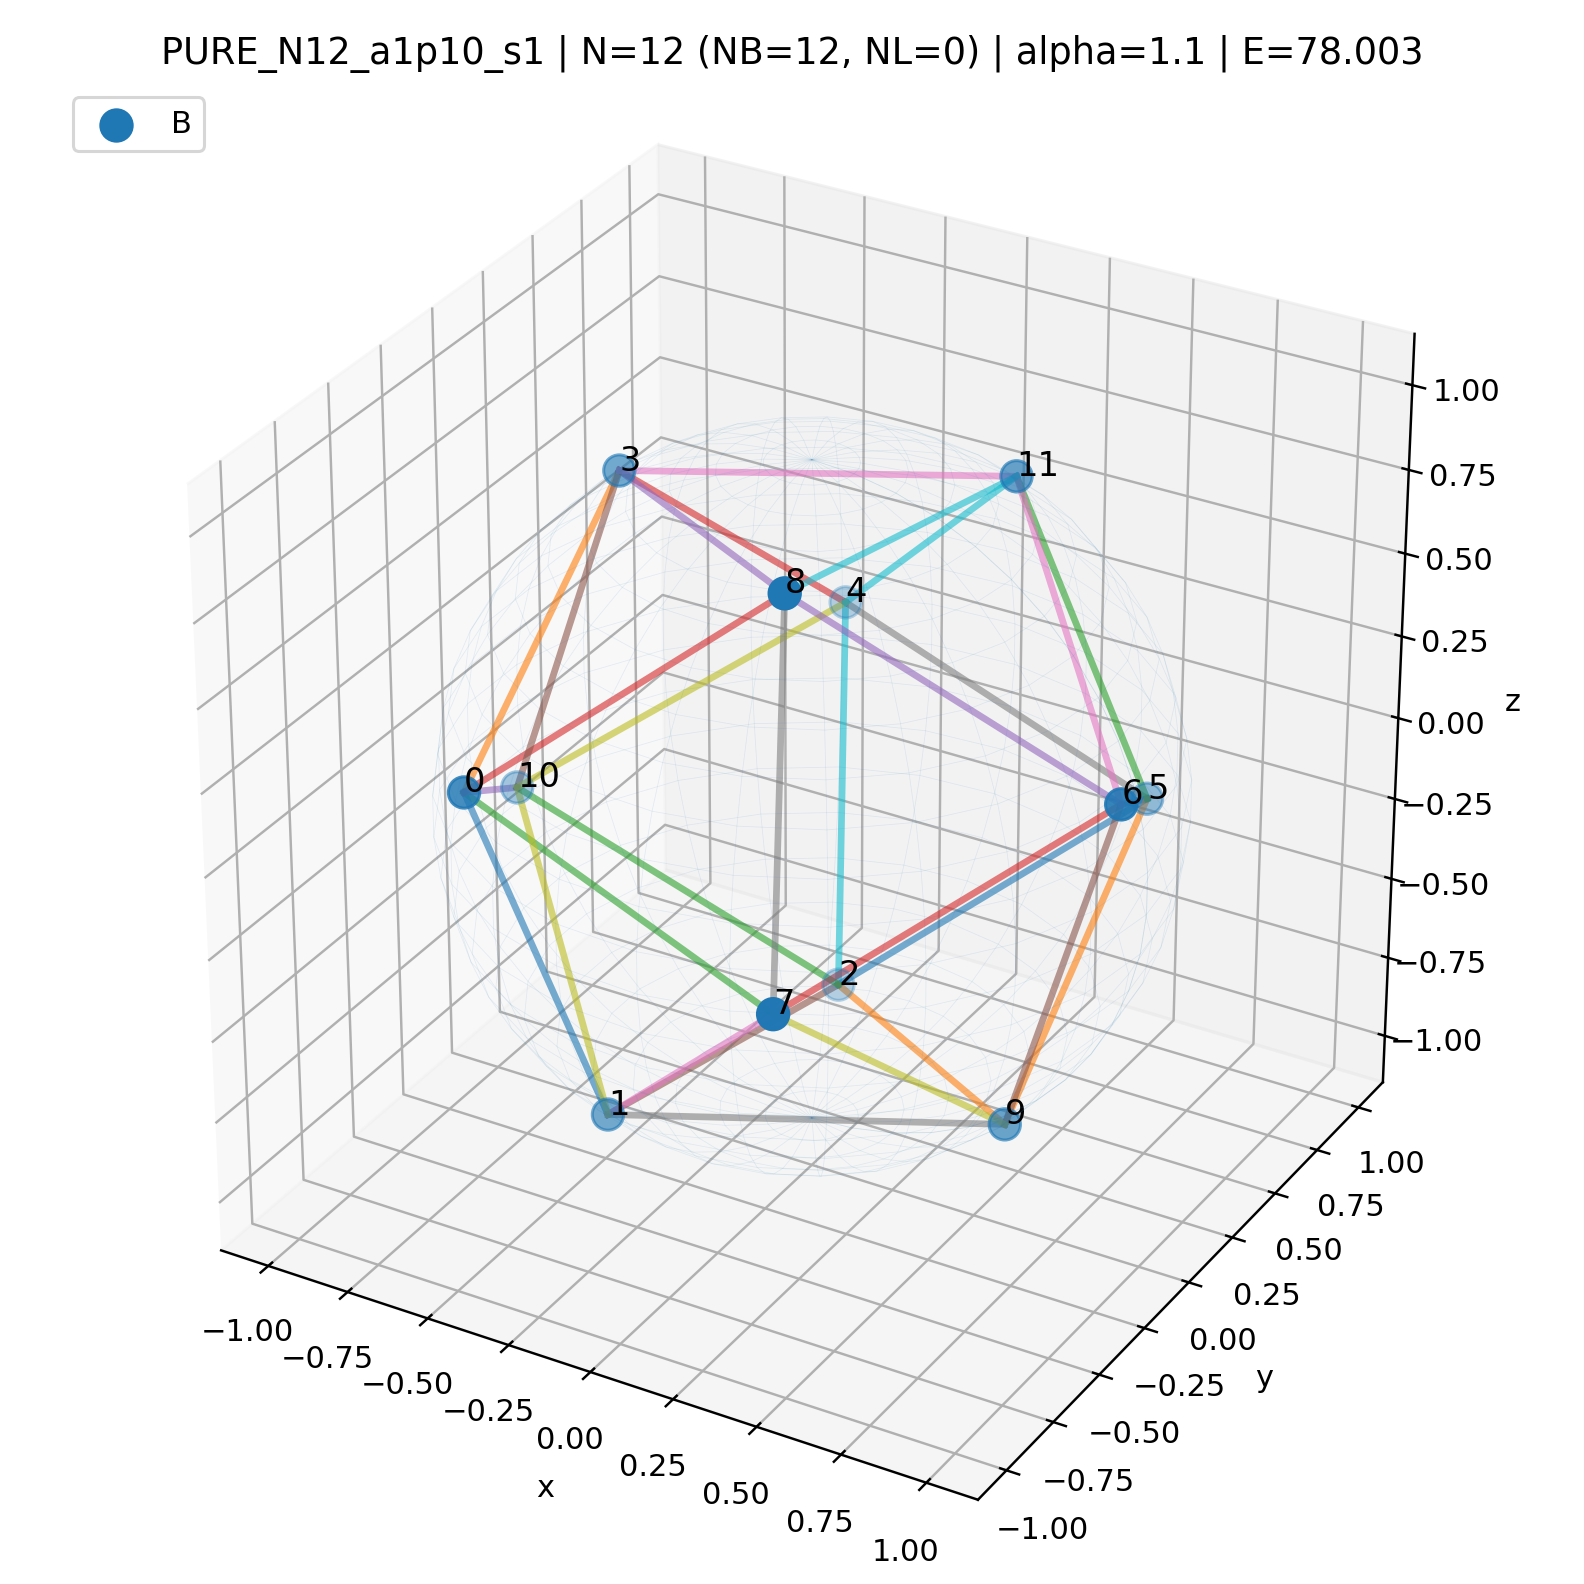
\includegraphics[width=0.82\textwidth]{figures/n12_icosahedral_probe_final.png}
\caption{Pure-$B$ probe for $N=12$. The optimized arrangement is consistent with an icosahedral-like packing and remains stable across the tested $\alpha$ values and seeds.}
    \label{fig:n12-probe}
\end{figure}

\section{Interpretation}
Taken together, the results define a coherent geometric sequence:
\begin{itemize}[leftmargin=1.5em]
    \item small-N baseline includes the tetrahedral form.
    \item $N=5$: trigonal bipyramidal form,
    \item $N=6$: soft octahedral regime,
    \item $N=7$: onset of geometric degeneracy and pentagonal motifs,
    \item $N=12$: stable icosahedral-like packing.
\end{itemize}

The significance of this sequence is methodological. Molecular-like geometries are not introduced as a table of allowed forms. They arise from a single optimization principle acting on nodes constrained to a sphere.

The model therefore suggests that a nontrivial part of the standard geometric repertoire may be recoverable from fewer assumptions than are usually introduced at the descriptive level.

\begin{table}[ht]
\centering
\caption{Compact summary of representative configurations in v.1 of the minimal sphere model.}
\label{tab:v1_summary}
\begin{tabular}{llll}
\hline
Case & Representative setting & Emergent motif & Interpretation \\
\hline
$N=5$ & $AX_2E_3$ & trigonal bipyramidal & reference rigid case \\
$N=6$ & $AX_2E_4$ & soft octahedral regime & stable but not perfectly rigid \\
$N=7$ & $AX_1E_6$ & shifted soft arrangement & onset of degeneracy \\
$N=7$ & $AX_3E_4$ & deformed structured form & soft geometric competition \\
$N=7$ & $AX_5E_2$ & pentagonal belt motif & strong pentagonal tendency \\
$N=12$ & pure-$B$ probe & icosahedral-like packing & robust high-symmetry packing \\
\hline
\end{tabular}
\end{table}

\section{Conclusion}
The value of the present model lies not in introducing a richer language, but in managing with fewer assumptions. Instead of separately postulating orbitals, hybridization patterns, and allowed molecular forms, the model starts from nodes, repulsion, spherical geometry, and energy minimization. Familiar forms then emerge as minima rather than as rules.

If this is a language, it is the simplest possible one: the language of energy minimization.

\section*{Reproducibility note}
A compact reproducibility bundle accompanies this paper, including representative JSON outputs, the N=6 map series, figure-generation scripts, summary data, and the LaTeX source.

\end{document}
